% Options for packages loaded elsewhere
% Options for packages loaded elsewhere
\PassOptionsToPackage{unicode}{hyperref}
\PassOptionsToPackage{hyphens}{url}
\PassOptionsToPackage{dvipsnames,svgnames,x11names}{xcolor}
%
\documentclass[
  authoryear,
  preprint]{elsarticle}
\usepackage{xcolor}
\usepackage{amsmath,amssymb}
\setcounter{secnumdepth}{5}
\usepackage{iftex}
\ifPDFTeX
  \usepackage[T1]{fontenc}
  \usepackage[utf8]{inputenc}
  \usepackage{textcomp} % provide euro and other symbols
\else % if luatex or xetex
  \usepackage{unicode-math} % this also loads fontspec
  \defaultfontfeatures{Scale=MatchLowercase}
  \defaultfontfeatures[\rmfamily]{Ligatures=TeX,Scale=1}
\fi
\usepackage{lmodern}
\ifPDFTeX\else
  % xetex/luatex font selection
\fi
% Use upquote if available, for straight quotes in verbatim environments
\IfFileExists{upquote.sty}{\usepackage{upquote}}{}
\IfFileExists{microtype.sty}{% use microtype if available
  \usepackage[]{microtype}
  \UseMicrotypeSet[protrusion]{basicmath} % disable protrusion for tt fonts
}{}
\makeatletter
\@ifundefined{KOMAClassName}{% if non-KOMA class
  \IfFileExists{parskip.sty}{%
    \usepackage{parskip}
  }{% else
    \setlength{\parindent}{0pt}
    \setlength{\parskip}{6pt plus 2pt minus 1pt}}
}{% if KOMA class
  \KOMAoptions{parskip=half}}
\makeatother
% Make \paragraph and \subparagraph free-standing
\makeatletter
\ifx\paragraph\undefined\else
  \let\oldparagraph\paragraph
  \renewcommand{\paragraph}{
    \@ifstar
      \xxxParagraphStar
      \xxxParagraphNoStar
  }
  \newcommand{\xxxParagraphStar}[1]{\oldparagraph*{#1}\mbox{}}
  \newcommand{\xxxParagraphNoStar}[1]{\oldparagraph{#1}\mbox{}}
\fi
\ifx\subparagraph\undefined\else
  \let\oldsubparagraph\subparagraph
  \renewcommand{\subparagraph}{
    \@ifstar
      \xxxSubParagraphStar
      \xxxSubParagraphNoStar
  }
  \newcommand{\xxxSubParagraphStar}[1]{\oldsubparagraph*{#1}\mbox{}}
  \newcommand{\xxxSubParagraphNoStar}[1]{\oldsubparagraph{#1}\mbox{}}
\fi
\makeatother


\usepackage{longtable,booktabs,array}
\newcounter{none} % for unnumbered tables
\usepackage{calc} % for calculating minipage widths
% Correct order of tables after \paragraph or \subparagraph
\usepackage{etoolbox}
\makeatletter
\patchcmd\longtable{\par}{\if@noskipsec\mbox{}\fi\par}{}{}
\makeatother
% Allow footnotes in longtable head/foot
\IfFileExists{footnotehyper.sty}{\usepackage{footnotehyper}}{\usepackage{footnote}}
\makesavenoteenv{longtable}
\usepackage{graphicx}
\makeatletter
\newsavebox\pandoc@box
\newcommand*\pandocbounded[1]{% scales image to fit in text height/width
  \sbox\pandoc@box{#1}%
  \Gscale@div\@tempa{\textheight}{\dimexpr\ht\pandoc@box+\dp\pandoc@box\relax}%
  \Gscale@div\@tempb{\linewidth}{\wd\pandoc@box}%
  \ifdim\@tempb\p@<\@tempa\p@\let\@tempa\@tempb\fi% select the smaller of both
  \ifdim\@tempa\p@<\p@\scalebox{\@tempa}{\usebox\pandoc@box}%
  \else\usebox{\pandoc@box}%
  \fi%
}
% Set default figure placement to htbp
\def\fps@figure{htbp}
\makeatother





\setlength{\emergencystretch}{3em} % prevent overfull lines

\providecommand{\tightlist}{%
  \setlength{\itemsep}{0pt}\setlength{\parskip}{0pt}}



 
\usepackage[]{natbib}
\bibliographystyle{elsarticle-harv}


\makeatletter
\@ifpackageloaded{caption}{}{\usepackage{caption}}
\AtBeginDocument{%
\ifdefined\contentsname
  \renewcommand*\contentsname{Table of contents}
\else
  \newcommand\contentsname{Table of contents}
\fi
\ifdefined\listfigurename
  \renewcommand*\listfigurename{List of Figures}
\else
  \newcommand\listfigurename{List of Figures}
\fi
\ifdefined\listtablename
  \renewcommand*\listtablename{List of Tables}
\else
  \newcommand\listtablename{List of Tables}
\fi
\ifdefined\figurename
  \renewcommand*\figurename{Figure}
\else
  \newcommand\figurename{Figure}
\fi
\ifdefined\tablename
  \renewcommand*\tablename{Table}
\else
  \newcommand\tablename{Table}
\fi
}
\@ifpackageloaded{float}{}{\usepackage{float}}
\floatstyle{ruled}
\@ifundefined{c@chapter}{\newfloat{codelisting}{h}{lop}}{\newfloat{codelisting}{h}{lop}[chapter]}
\floatname{codelisting}{Listing}
\newcommand*\listoflistings{\listof{codelisting}{List of Listings}}
\makeatother
\makeatletter
\makeatother
\makeatletter
\@ifpackageloaded{caption}{}{\usepackage{caption}}
\@ifpackageloaded{subcaption}{}{\usepackage{subcaption}}
\makeatother
\journal{Journal Name}
\usepackage{bookmark}
\IfFileExists{xurl.sty}{\usepackage{xurl}}{} % add URL line breaks if available
\urlstyle{same}
\hypersetup{
  pdftitle={An Introduction to Reinforcement Learning},
  pdfauthor={Caleb Lee, Catherine Cao, Arshia Mago, Ashlee King, Christina Fan},
  pdfkeywords={Q-learning, Reinforcement
learning, State, Agent, Action, TD learning},
  colorlinks=true,
  linkcolor={blue},
  filecolor={Maroon},
  citecolor={Blue},
  urlcolor={Blue},
  pdfcreator={LaTeX via pandoc}}


\setlength{\parindent}{6pt}
\begin{document}

\begin{frontmatter}
\title{An Introduction to Reinforcement Learning}
\author[1]{Caleb Lee, Catherine Cao, Arshia Mago, Ashlee King, Christina
Fan%
%
}


\affiliation[1]{organization={University of Waterloo, Department of
Psychology},addressline={200 University Avenue
West},city={Waterloo},postcode={N2L 3G1},postcodesep={}}

\cortext[cor1]{Corresponding author}

        
\begin{abstract}
This is the abstract. Lorem ipsum dolor sit amet, consectetur adipiscing
elit. Vestibulum augue turpis, dictum non malesuada a, volutpat eget
velit. Nam placerat turpis purus, eu tristique ex tincidunt et. Mauris
sed augue eget turpis ultrices tincidunt. Sed et mi in leo porta
egestas. Aliquam non laoreet velit. Nunc quis ex vitae eros aliquet
auctor nec ac libero. Duis laoreet sapien eu mi luctus, in bibendum leo
molestie. Sed hendrerit diam diam, ac dapibus nisl volutpat vitae.
Aliquam bibendum varius libero, eu efficitur justo rutrum at. Sed at
tempus elit.
\end{abstract}





\begin{keyword}
    Q-learning \sep Reinforcement
learning \sep State \sep Agent \sep Action \sep 
    TD learning
\end{keyword}
\end{frontmatter}
    

\section{Introduction}\label{introduction}

\subsection{History}\label{history}

\begin{itemize}
\tightlist
\item
  Ashlee History
\end{itemize}

\subsection{Importance and
Applications}\label{importance-and-applications}

\begin{itemize}
\tightlist
\item
  Arshia + some Catherine applications stuff \textless!-- Here are two
  sample references: \citet{Feynman1963118} \citet{Dirac1953888}.
\end{itemize}

With this template using elsevier class, natbib will be used. Three
bibliographic style files (*.bst) are provided and their use controled by
\texttt{cite-style} option:

\begin{itemize}
\tightlist
\item
  \texttt{citestyle:\ number} (default) will use
  \texttt{elsarticle-num.bst} - can be used for the numbered scheme
\item
  \texttt{citestyle:\ numbername} will use
  \texttt{elsarticle-num-names.bst} - can be used for numbered with new
  options of natbib.sty
\item
  \texttt{citestyle:\ authoryear} will use \texttt{elsarticle-harv.bst}
  --- can be used for author year scheme
\end{itemize}

This \texttt{citestyle} will insert the right \texttt{.bst} and set the
correct \texttt{classoption} for \texttt{elsarticle} document class.

Using \texttt{natbiboptions} variable in YAML header, you can set more
options for \texttt{natbib} itself . Example

\texttt{yaml\ natbiboptions:\ longnamesfirst,angle,semicolon}
--\textgreater{}

\section{Mathematical Theory}\label{mathematical-theory}

\subsection{Markov Decision Process}\label{markov-decision-process}

The Markov Decision Process (MDP) forms the mathematical foundation of
reinforcement learning (RL) algorithms. It provides a framework for
modeling sequential decision-making problems in stochastic environments,
where an agent's actions influence both immediate rewards and subsequent
states. These systems satisfy Markov property, meaning that the state
transition and reward depend only on the current state and action,
regardless of the prior process.

A MDP is defined by states, actions and rewards, which together describe
the interaction between an agent and its environment. The set of all
possible states is denoted by \(\mathcal{S}\), where each state \(S_t\)
represents specific coordinates or condition of the environment at time
step t. The agent observes the current state \(S_t\) and selects an
action \(A_t\), where \(\mathcal{A}(s)\) denotes the set of available
actions in that state.

After taking action \(A_t\), the agent transitions to a new state
\(S_{t+1}\). The state transition probability is the likelihood of
transitioning to a subsequent state \(s'\) given the current
state-action pair \((s, a)\): \[
P(S' \mid s, a) = \Pr(S_{t+1} = S' \mid S_t = s, A_t = a)
\] Simultaneously, the agent receives an expected immediate reward
\(R(s, a)\), which is defined as the expected reward received after
taking action \(A\) in state \(S\): \[
R(s,a) = \mathbb{E}\left[ R_{t+1} \mid S_t = s, A_t = a \right]
\]

\subsection{Policy and Value Function}\label{policy-and-value-function}

A policy, denoted as \(\pi\), specifies agent's behaviour by defining
how actions are selected in each state,
\(\pi(a \mid s) = \Pr(A_t = a \mid S_t = s)\) represents the probability
that the agent selects action \(a\) when in state \(s\).The state-value
function, \(v_\pi(s)\), represents the expected cumulative reward
received when the agent starts in state s and follows policy \(\pi\). It
is defined as: \[
v_\pi(s) = \mathbb{E}_\pi \left[ \sum_{k=0}^{\infty} \gamma^k R_{t+k+1} \,\middle|\, S_t = s \right]
\] where \(\gamma \in [0, 1]\) is the discount factor, which balances
immediate reward and the long-term reward. A smaller γ gives more weight
to immediate rewards, while a γ closer to 1 gives more weight to
long-term rewards.

To evaluate the value of specific actions taken in a state, we use the
action-value function (or Q-function), \(q_\pi(s,a)\). This function
measures the expected cumulative reward when the agent starts in state
\(s\), takes action \(a\), and follows policy \(\pi\): \[
q_\pi(s,a) = \mathbb{E}_\pi \left[ \sum_{k=0}^{\infty} \gamma^k R_{t+k+1} \,\middle|\, S_t = s, A_t = a \right]
\]

\subsection{Bellman Equation}\label{bellman-equation}

The Bellman equation for \(v_\pi\) shows a recursive relationship
between the value of a state and the values of subsequent states. It
describes the value of a state as the sum of the expected immediate
reward and the discounted value of subsequent states. For any policy
\(\pi\), the state-value function satisfies: \[
v_\pi(s) = \sum_a \pi(a \mid s) \sum_{s',r} p(s',r \mid s,a)\left[ r + \gamma v_\pi(s') \right]
\]

The Bellman optimality equation can be expressed without reference to a
specific policy \(\pi\), instead selecting the best possible action. The
Bellman optimality equation for the optimal state-value function is: \[
v^*(s) = \max_{a \in \mathcal{A}(s)} \sum_{s',r} p(s',r \mid s,a)\left[ r + \gamma v^*(s') \right]
\] It states that the optimal value of a state is the maximum expected
total reward achievable by choosing the best action, and assuming
optimal behaviour in subsequent states. The Bellman optimality equation
for the optimal action-value function states the optimal value of a
action-state pair: \[
q^*(s,a) = \sum_{s',r} p(s',r \mid s,a)\left[ r + \gamma \max_{a'} q^*(s',a') \right]
\] It represents the maximum expected total reward obtained by taking
action \(a\) in state \(s\), followed by optimal behaviour thereafter.
It forms the foundation for Q-learning algorithm.

\subsection{Q-Learning}\label{q-learning}

A model of the environment refers to any mechanism that allows the agent
to predict the outcome of its actions. Reinforcement learning methods
can be categorized into model-based and model-free methods, depending on
whether the agent has access to a model of the environment. Model-based
agents utilize planning, which is a computational process that uses a
model to improve a policy. The agent uses its model to generate
simulated experience and evaluate future trajectories. In contrast,
model-free agents learn directly from real experience by interacting
with the environment, executing actions and observing outcomes.

Q-learning is categorized as a model-free, off-policy algorithm. The
primary goal of off-policy learning is to evaluate and optimize a target
policy, which is the strategy intended to become optimal.
Simultaneously, the agent follows a distinct, more exploratory behaviour
policy to interact with the environment. The \(\epsilon\)-greedy policy
is used in Q-learning to select an action, which balances the trade-off
between exploration and exploitation. With probability of \(\epsilon\),
the agent explores by selecting a random action (or the non-greedy
action) to improve its estimates of the optimal values. With probability
\(1 - \epsilon\), the agent exploits its current knowledge by choosing
the greedy action, which is the action with the highest current
estimated value.

Q-learning is a Temporal-Difference (TD) control algorithm that directly
approximates the optimal action-value function. TD error, \(\delta_t\),
represents the discrepancy between the current estimate of \(Q\)-value
and the updated estimate of future value from the next state: \[
\delta_t = R_{t+1} + \gamma Q(S_{t+1}, a') - Q(S_t, A_t)
\] The Q-learning update rule utilizes this error to refine its
estimates: \[
Q(S_t, A_t) \leftarrow Q(S_t, A_t) + \alpha \left[ R_{t+1} + \gamma \max_a Q(S_{t+1}, a) - Q(S_t, A_t) \right]
\] where \(\alpha \in [0, 1]\) is the learning rate (or step-size
parameter). The \(Q\)-value \(Q(S_t, A_t)\) is the current estimate of
the value of taking action \(A\) in state \(S\). It is updated by
incorporating the immediate reward and the discounted value of the best
possible action in the subsequent state. This update assumes that the
agent follows the optimal policy from the next state onward. As the
estimates converge to the optimal values (\(Q^*\)), the optimal policy
\(\pi^*\) can be obtained by selecting the action that maximizes this
value: \(\pi^*(x) = \arg\max_{a} Q^*(x, a)\).

\section{Methods}\label{methods}

\begin{itemize}
\tightlist
\item
  Christina and Caleb \#\# Implementation We built and implemented a
  Q-learning algorithm within a maze environment. The environment was
  represented as a 6 × 6 grid constructed using a NumPy array, where
  integer values encoded state types and associated rewards.
  Specifically, cells were defined as follows: 0 represented empty
  traversable space, 1 represented impassable walls, 2 represented fatal
  states (``holes'') that returned the agent to the starting position,
  and 3 represented the goal state associated with a positive reward and
  episode termination.
\end{itemize}

A Q-table was initialized with zeros to represent the expected value of
each state--action pair. The learning rate (α), future discount factor
(γ), and exploration rate (ε) were predefined and held constant
throughout training. The agent's action space consisted of four discrete
movements (up, down, left, right).

At each step, the agent selected an action using the Epsilon-Greedy
strategy. State transitions were determined by applying the selected
action to the agent's current position, with resulting coordinates
mapped onto the grid to determine the subsequent state and corresponding
reward.

Q-values were iteratively updated using the temporal difference learning
rule based on the observed reward and the maximum expected future reward
from the subsequent state. Training was conducted over a fixed number of
episodes, with each episode beginning at the starting state and
terminating upon reaching the goal or a terminal penalty state.

\subsection{Neuropsychiatry Extension}\label{neuropsychiatry-extension}

\begin{itemize}
\tightlist
\item
  Caleb Part
\item
  Q learning in computational psychiatry
\item
  Example: D1/D2 receptors
\end{itemize}

\section{Results}\label{results}

\subsection{Model}\label{model}

After running 1000 episodes, we present evidence of the agent's learning
process. Figure~\ref{fig-stepsep} illustrates changes in the number of
steps the agent takes to complete one episode over the course of 500
episodes.

\begin{figure}[H]

\centering{

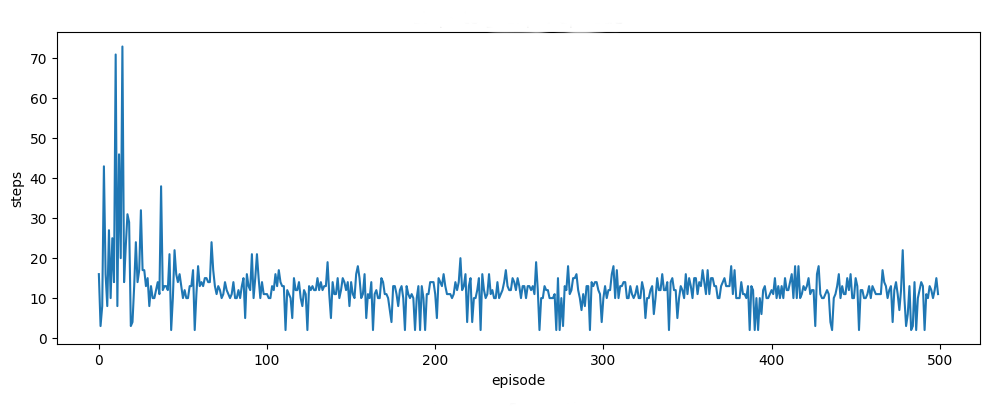
\includegraphics[width=0.85\linewidth,height=\textheight,keepaspectratio]{images/stepsep.png}

}

\caption{\label{fig-stepsep}Changes in Steps to Complete One Episode}

\end{figure}%

Figure~\ref{fig-delta} presents changes in the TD learning error (delta)
over time across 6000 episodes.

\begin{figure}[H]

\centering{

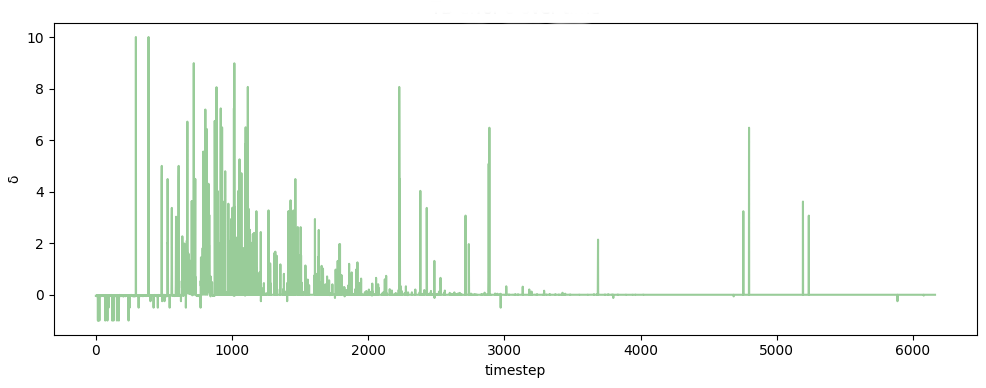
\includegraphics[width=0.85\linewidth,height=\textheight,keepaspectratio]{images/delta.png}

}

\caption{\label{fig-delta}TD Error Over Time}

\end{figure}%

Figure~\ref{fig-heatmap} is a Q-value heatmap showing the Q values of
the best action to take in a given state (i.e.~state-action pair that
renders the maximal Q-value), with greater Q-values of darker color.

\begin{figure}[H]

\centering{

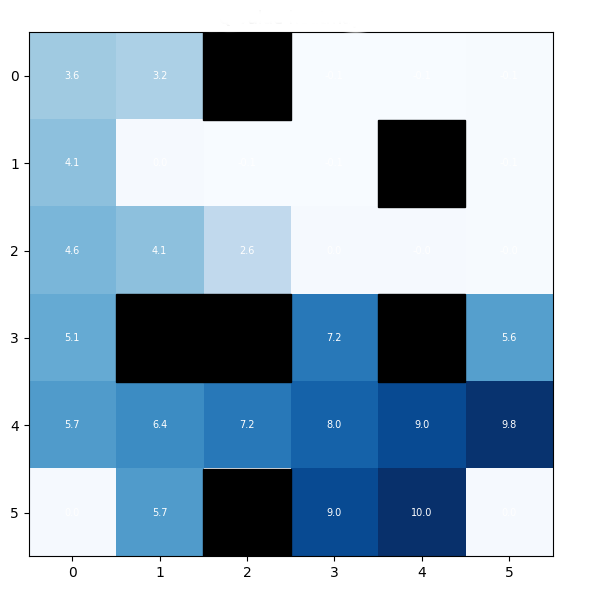
\includegraphics[width=0.85\linewidth,height=\textheight,keepaspectratio]{images/heatmap.png}

}

\caption{\label{fig-heatmap}Q-Value Heatmap}

\end{figure}%

Figure~\ref{fig-policy} illustrates the optimal actions to take in a
given state, with visualizations of actions as arrows in the maze
environment. This represents the optimal policy the agent is learning.

\begin{figure}[H]

\centering{

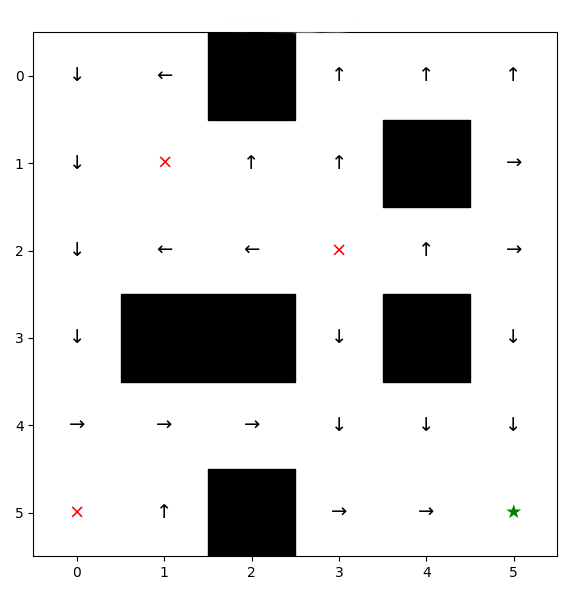
\includegraphics[width=0.85\linewidth,height=\textheight,keepaspectratio]{images/policy.png}

}

\caption{\label{fig-policy}Optimal Learned Policy}

\end{figure}%

\subsection{Neuropsychiatry
Extension}\label{neuropsychiatry-extension-1}

\begin{itemize}
\tightlist
\item
  Caleb
\end{itemize}


\renewcommand\refname{References}
\bibliography{bibliography.bib}



\end{document}
